%\documentclass{article}
%\usepackage[utf8]{inputenc}
\documentclass[apj,twocolumn]{aastex631}
\usepackage{graphicx,here,comment}

\begin{document}

\title{SDSS-GAIA Calibration Note}
\author{GAIA-SDSS Friends}

\begin{abstract}
Calibration is hard
\end{abstract}

%\title{Probing Dark Galaxies through Type Ia Supernovae}
%\author{Nao Suzuki}
%\date{February 2021}
%\usepackage{graphicx}
%\begin{document}
%\maketitle

\section{GAIA DR3}
GAIA DR3 is released in June 2022.   We aim to take advantage of GAIA data, and calibrate SDSS spectra.  We use SDSS DR17, v5-13-2 reduction and SDSS DR8.  Note, DR17 and DR8 does not share the data set.

\section{Basic Statistics}
In 'spobj\_dr8.fits', 1,843,200 objects are listed, but some do not have thing\_id, and we are missing 130,391 objects.
DR17, spall file contains 3,948,000 spectra, but if we exclude thing\_id=-1, 406,483 objects are dropped out.
We note, we have a more stellar spectra in DR8 than DR17.

We collected GAIA XP spectra which is a low resolution spectra and becomes public for the first time in June 2022.  In the second half of Table \ref{tbl:summary}, we summarize the number statistics of objects which has both GAIA XP and SDSS spectra.

\begin{deluxetable*}{rrrrrrr}[ht]
\label{tbl:summary}
\title{GAIA-SDSS Spectra Summary}
\tablecaption{Top half shows the number of spectra for DR8 and DR17.  The second half shows the number of GAIA XP spectra which has SDSS spectra}
\tablehead{
\colhead{Survey}&
\colhead{Number of Plates}&
\colhead{Number of Spectra}&
\colhead{Missing}&
\colhead{Star}&
\colhead{Quasar}&
\colhead{Galaxy}
}
\startdata
SDSS-DR8 & 3,685 & 1,712,809 & 130,391 & 605,884& 142,232& 964,693\\
SDSS-DR17 & 4,131 & 3,541,517 & 406,483 & 499,127 & 963,616 & 2,078,774\\
\hline
GAIAXP-DR8 & 2,782 & 272,729&  & 240,470& 32,259 & N/A \\
GAIAXP-DR17 & 3,950 & 88,915  &  & 63,083 & 25,832 & N/A
\enddata
\end{deluxetable*}



\begin{figure*}%[ht]
\begin{center}
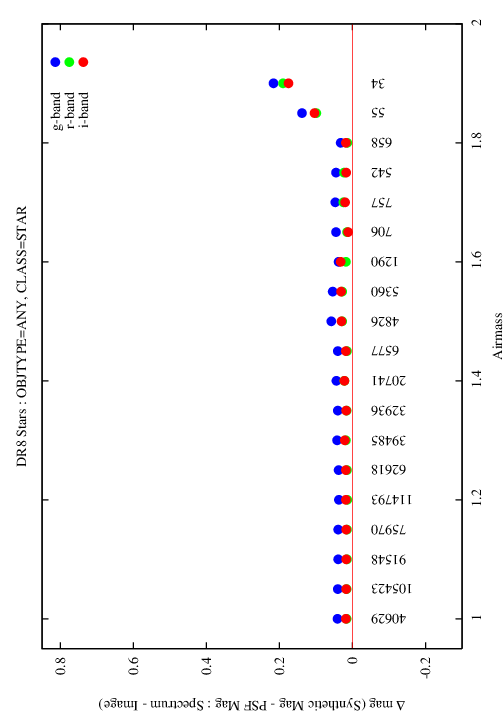
\includegraphics[angle=270,width=8.9cm]{figures/120821_01_airmass_vs_dmag_star_dr8.png}
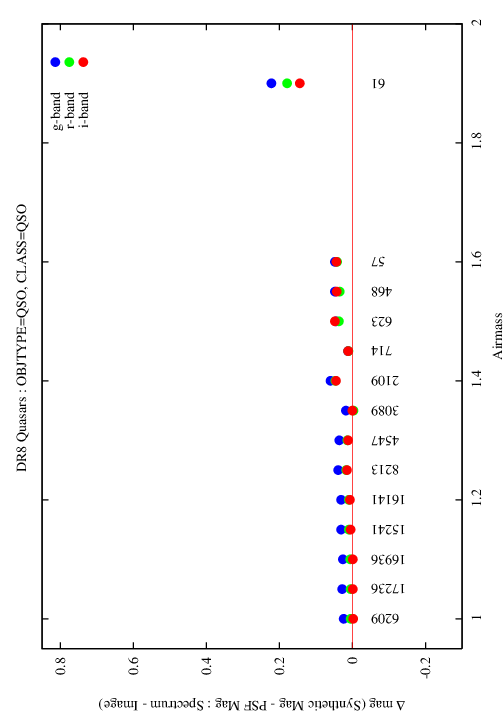
\includegraphics[angle=270,width=8.9cm]{figures/120821_04_airmass_vs_dmag_quasar_dr8.png}
\caption{DR8: Comparison of Synthetic Magnitude from Model Spectrum and PSF magnitude as a function of airmass. Stars and Quasars are shown left and right respectively.  We do not see any trend, and in general, spectra are well flux calibrated.}
\end{center}
\end{figure*}

\begin{figure*}%[ht]
\begin{center}
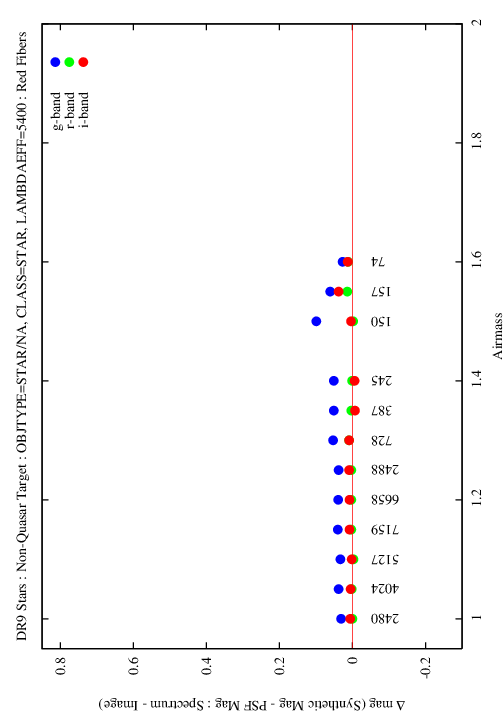
\includegraphics[angle=270,width=8.9cm]{figures/120821_02_airmass_vs_dmag_star_dr9_redfiber.png}
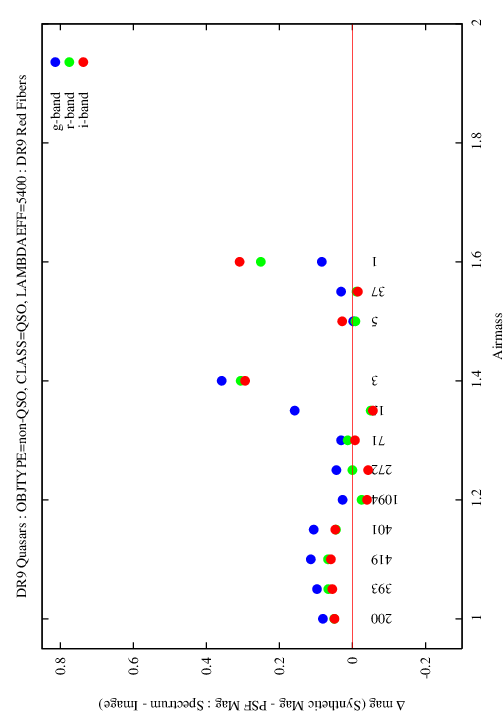
\includegraphics[angle=270,width=8.9cm]{figures/120821_05_airmass_vs_dmag_quasar_dr9_redfibers.png}
\caption{DR9 lambda$\_$eff=5400 : Starting SDSS-III, spectrograph is upgraded.  To enhance S/N in blue, a slight offset of fiber position is introduced as well as washers.  Two fiber positions are named lambda$\_$eff=4000 and 5400.  What is shown here is the case for lambda$\_$eff=5400 which is the same as SDSS DR8.}
\end{center}
\end{figure*}

\begin{figure*}%[ht]
\begin{center}
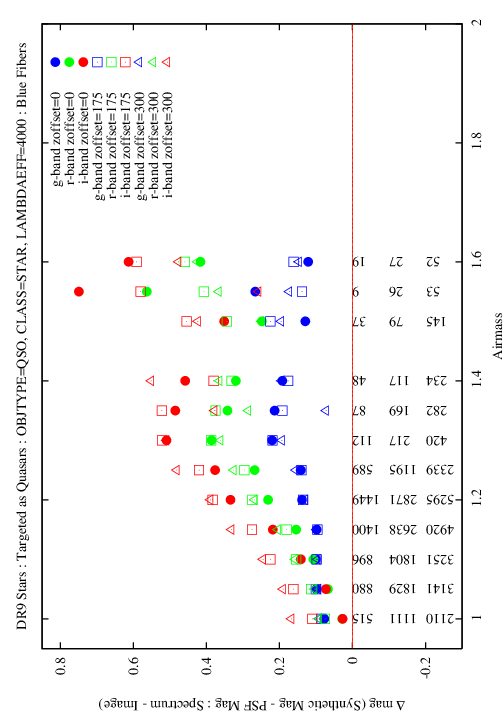
\includegraphics[angle=270,width=8.9cm]{figures/120821_03_airmass_vs_dmag_star_dr9_bluefiber.png}
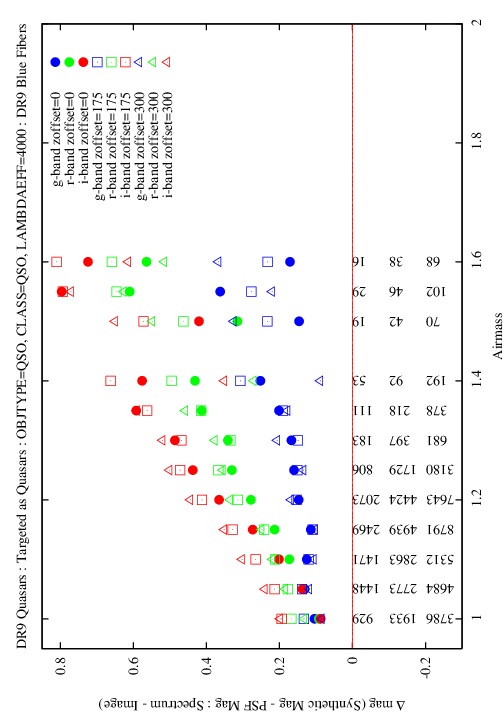
\includegraphics[angle=270,width=8.9cm]{figures/120821_06_airmass_vs_dmag_quasar_dr9_bluefiber.png}
\caption{DR9 lambda$\_$eff=4000 : Now, the problem emerges. Enhancing S/N in blue sacrifices the flux calibration.  Washer has 3 layers, z=0, z=175, and z=300 from inner part to outskirts.  When elevation is low, namely airmass is high, hour angle difference becomes eminent, and flux calibration gets difficult.}
\end{center}
\end{figure*}


\begin{figure*}%[ht]
\begin{center}
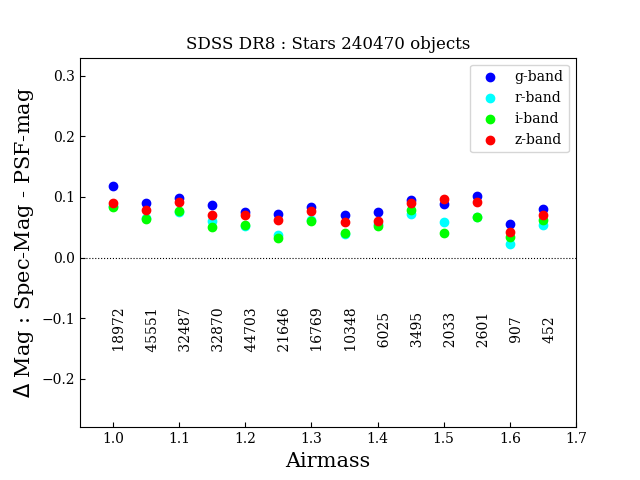
\includegraphics[angle=0,width=8.9cm]{figures/20220810_airmass_vs_dmag_dr8star.png}
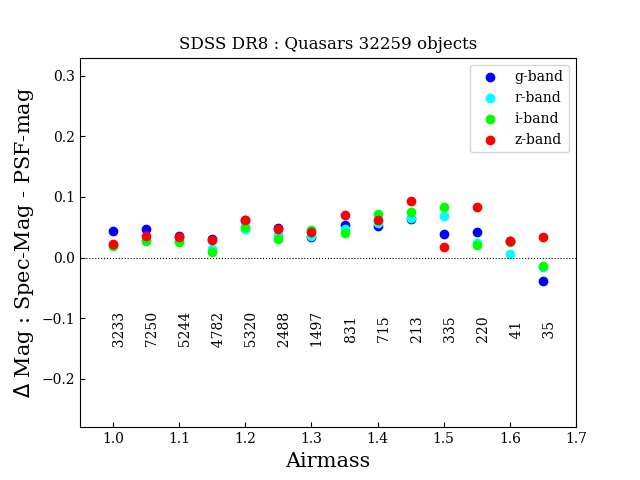
\includegraphics[angle=0,width=8.9cm]{figures/20220810_airmass_vs_dmag_dr8quasar.png}
\caption{DR8 : Now we do the test again.  This time, we compare synthesized mag from the observed spectra.  Note the ones above are synthesized mag from the best model spectra. Several percent offset, but not too bad. Stars left, and Quasars right.}
\end{center}
\end{figure*}

\begin{figure*}%[ht]
\begin{center}
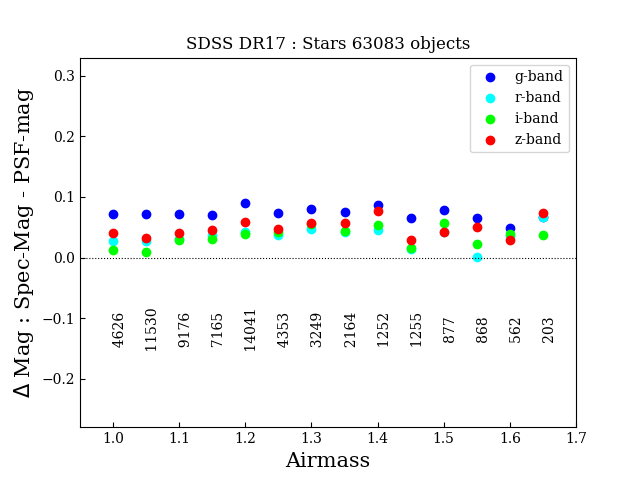
\includegraphics[angle=0,width=8.9cm]{figures/20220810_airmass_vs_dmag_dr17star.png}
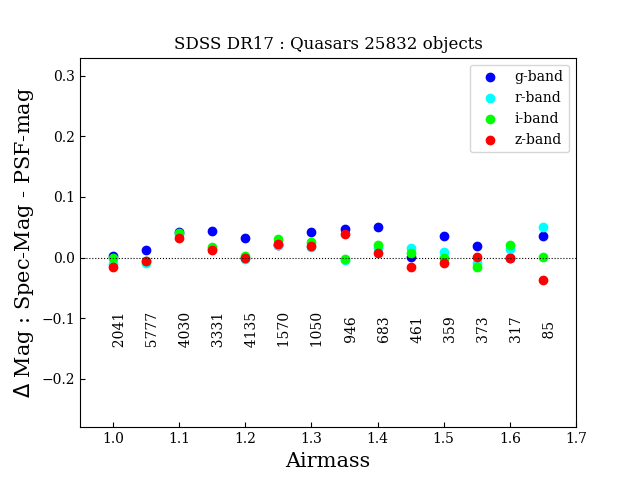
\includegraphics[angle=0,width=8.9cm]{figures/20220810_airmass_vs_dmag_dr17quasar.png}
\caption{DR17 : Now SDSS-III/IV data are being calibrated by Daniel Margala's method.  It has greatly imporved the flux calibration.}
\end{center}
\end{figure*}


\begin{figure*}%[ht]
\begin{center}
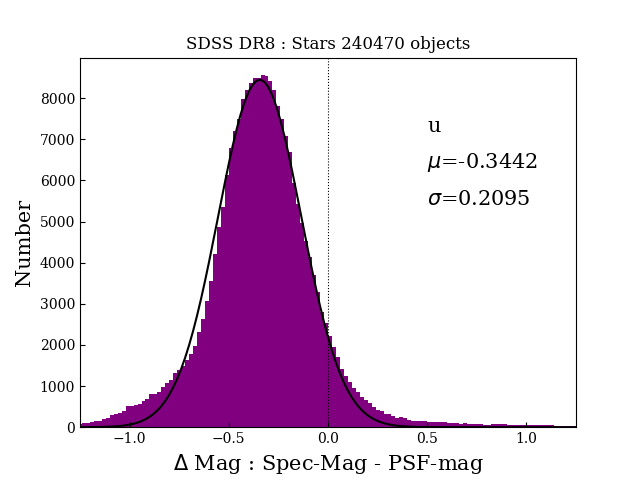
\includegraphics[angle=0,width=3.5cm]{figures/20220811_dmag_histogram_u_dr8stars.png}
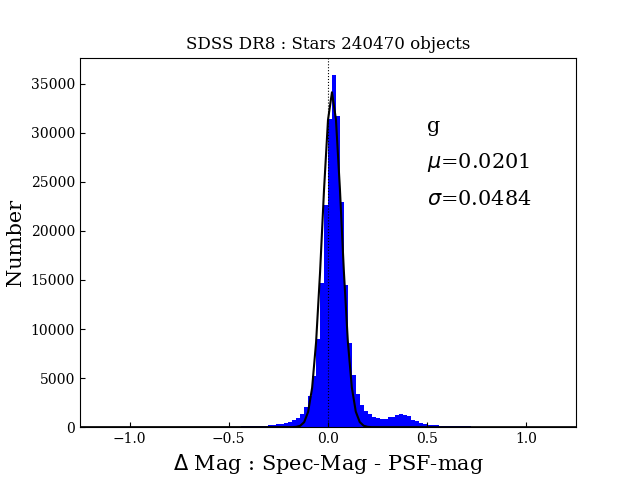
\includegraphics[angle=0,width=3.5cm]{figures/20220811_dmag_histogram_g_dr8stars.png}
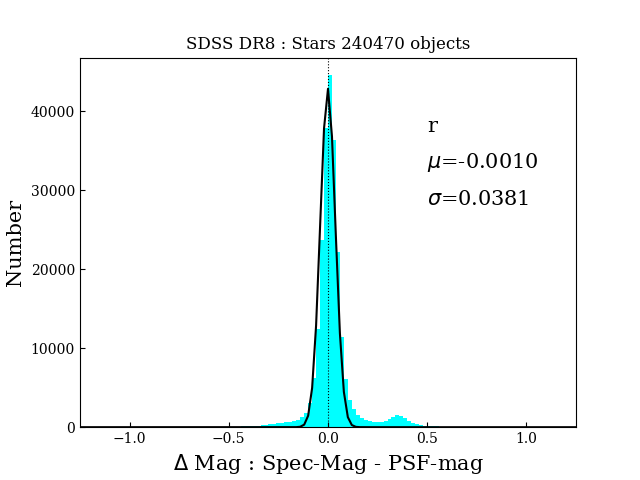
\includegraphics[angle=0,width=3.5cm]{figures/20220811_dmag_histogram_r_dr8stars.png}
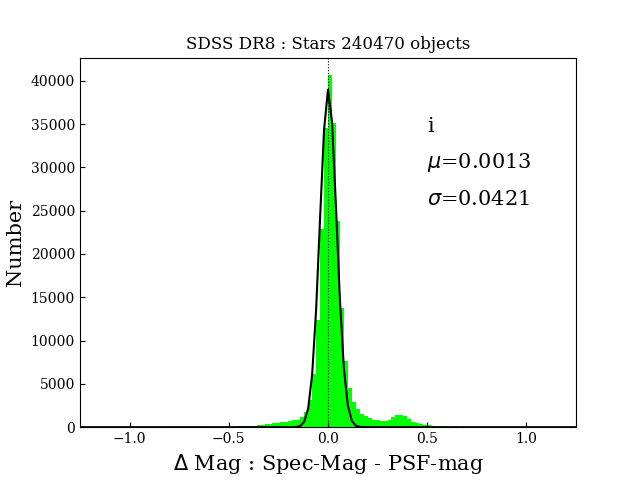
\includegraphics[angle=0,width=3.5cm]{figures/20220811_dmag_histogram_i_dr8stars.png}
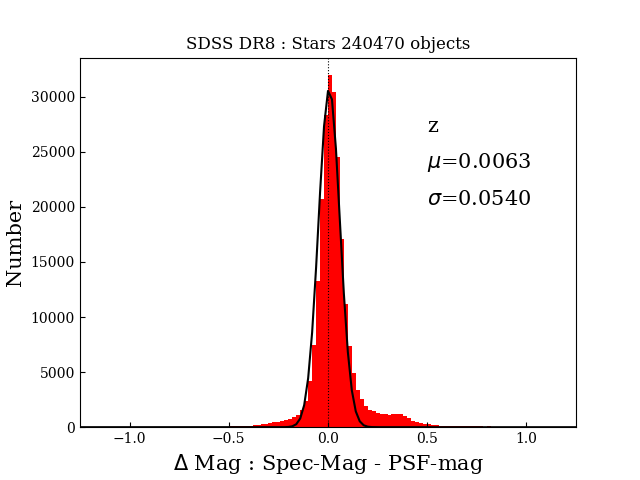
\includegraphics[angle=0,width=3.5cm]{figures/20220811_dmag_histogram_z_dr8stars.png}
\caption{DR8 Star: Histogram of synthesized magnitude from spectra vs PSF magnitude.
u-band shows a large offset but it is due to spectral wavelength does not cover entire u-band region.}
\end{center}
\end{figure*}

\begin{figure*}%[ht]
\begin{center}
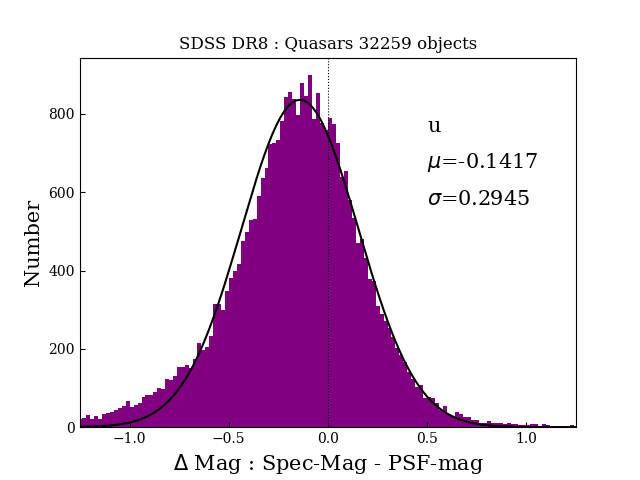
\includegraphics[angle=0,width=3.5cm]{figures/20220811_dmag_histogram_u_dr8quasars.png}
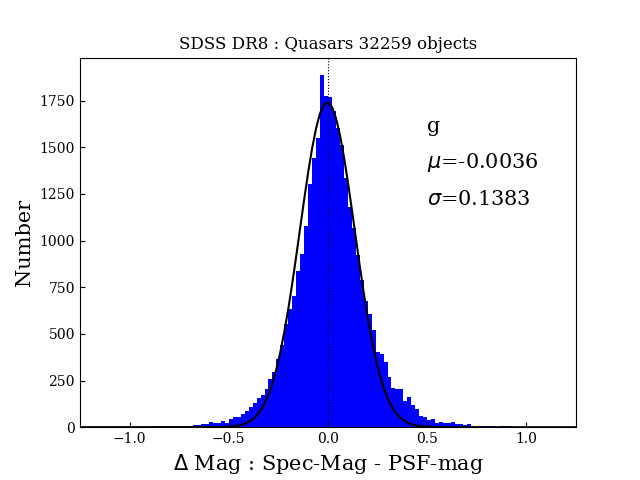
\includegraphics[angle=0,width=3.5cm]{figures/20220811_dmag_histogram_g_dr8quasars.png}
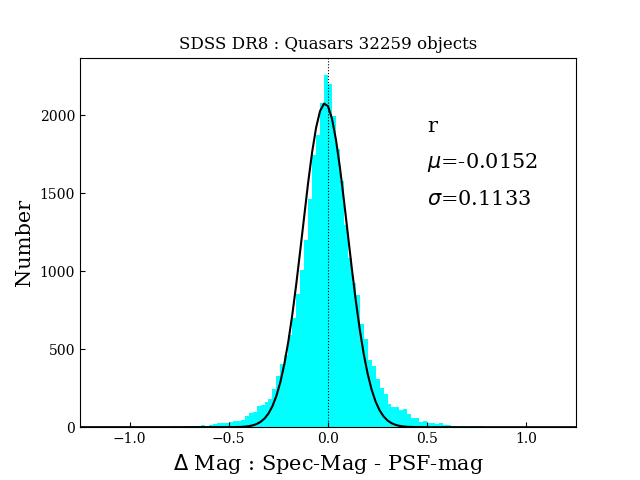
\includegraphics[angle=0,width=3.5cm]{figures/20220811_dmag_histogram_r_dr8quasars.png}
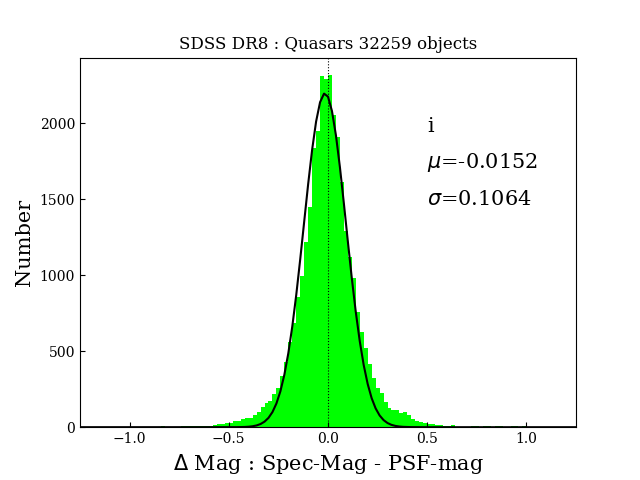
\includegraphics[angle=0,width=3.5cm]{figures/20220811_dmag_histogram_i_dr8quasars.png}
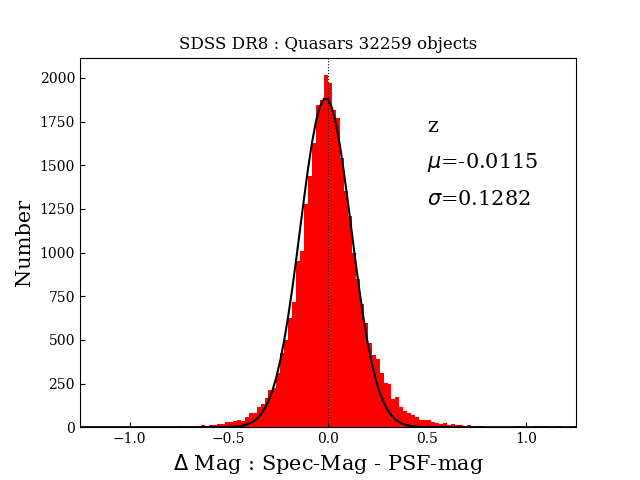
\includegraphics[angle=0,width=3.5cm]{figures/20220811_dmag_histogram_z_dr8quasars.png}
\caption{DR8 Quasar: Histogram of synthesized magnitude from spectra vs PSF magnitude.
u-band shows a large offset but it is due to spectral wavelength does not cover entire u-band region.}
\end{center}
\end{figure*}

\begin{figure*}%[ht]
\begin{center}
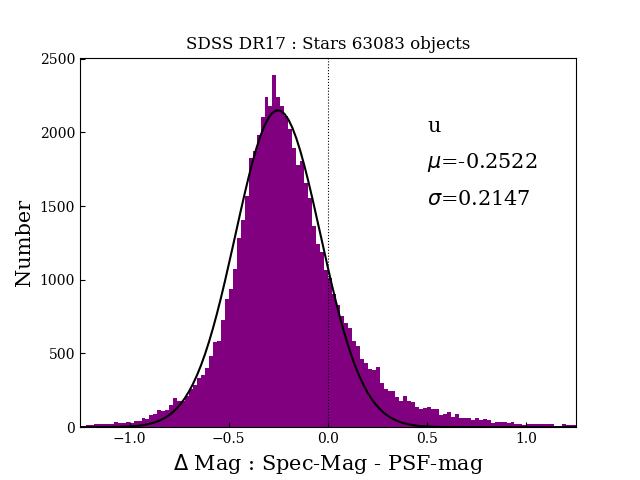
\includegraphics[angle=0,width=3.5cm]{figures/20220811_dmag_histogram_u_dr17stars.png}
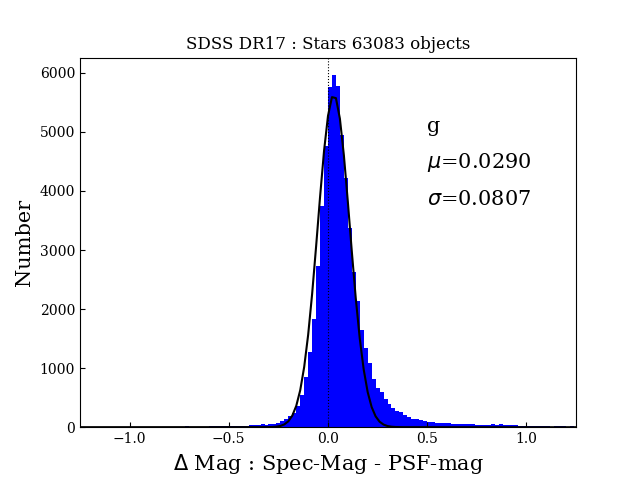
\includegraphics[angle=0,width=3.5cm]{figures/20220811_dmag_histogram_g_dr17stars.png}
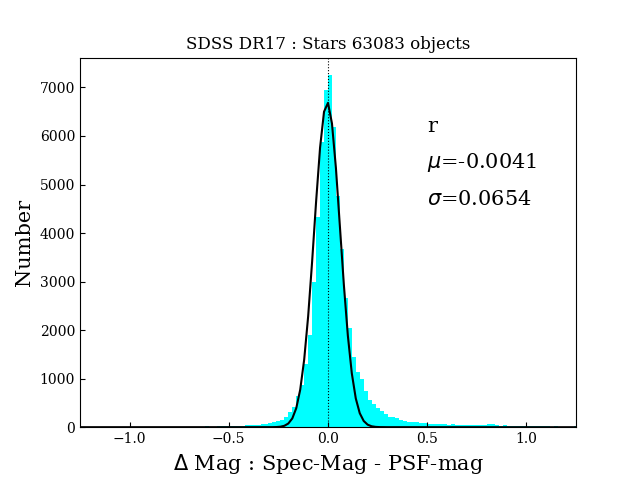
\includegraphics[angle=0,width=3.5cm]{figures/20220811_dmag_histogram_r_dr17stars.png}
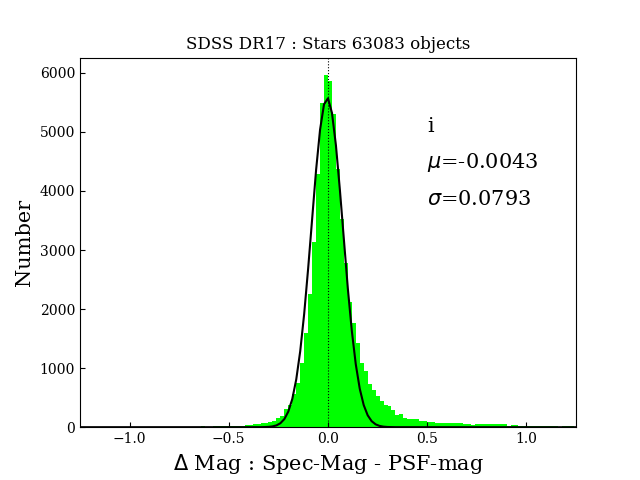
\includegraphics[angle=0,width=3.5cm]{figures/20220811_dmag_histogram_i_dr17stars.png}
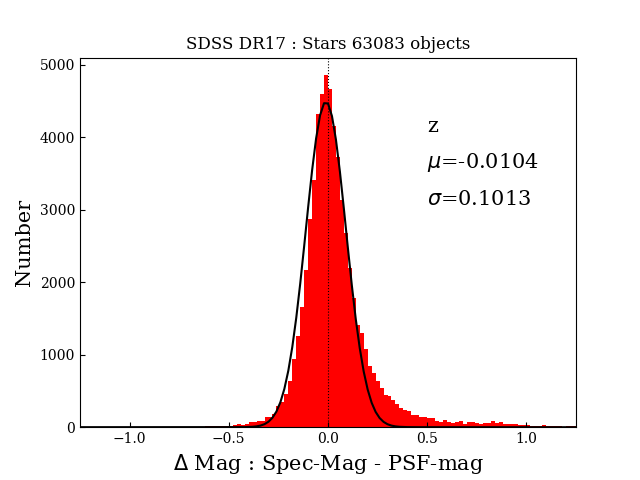
\includegraphics[angle=0,width=3.5cm]{figures/20220811_dmag_histogram_z_dr17stars.png}
\caption{DR17 Star: Histogram of synthesized magnitude from spectra vs PSF magnitude.
u-band shows a large offset but it is due to spectral wavelength does not cover entire u-band region.}
\end{center}
\end{figure*}


\begin{figure*}%[ht]
\begin{center}
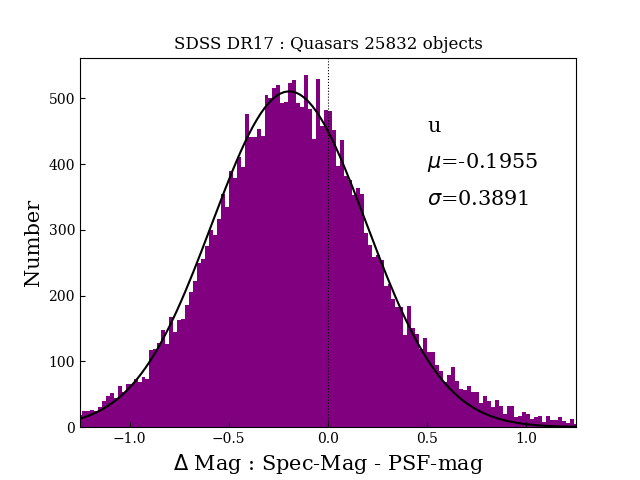
\includegraphics[angle=0,width=3.5cm]{figures/20220811_dmag_histogram_u_dr17quasars.png}
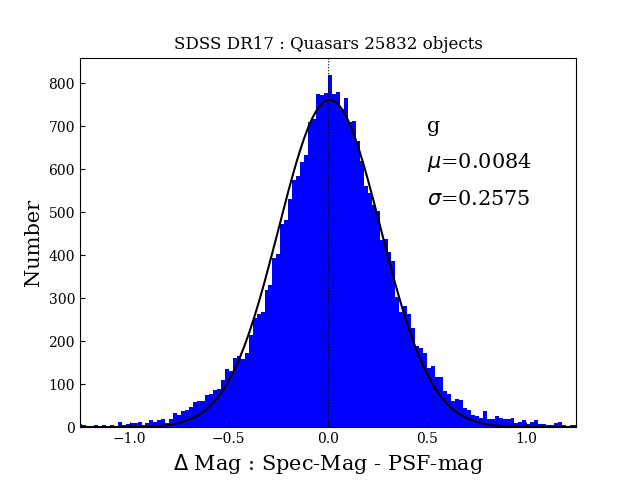
\includegraphics[angle=0,width=3.5cm]{figures/20220811_dmag_histogram_g_dr17quasars.png}
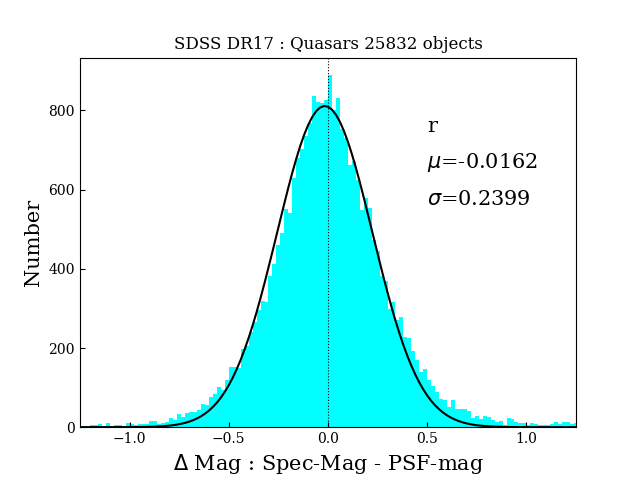
\includegraphics[angle=0,width=3.5cm]{figures/20220811_dmag_histogram_r_dr17quasars.png}
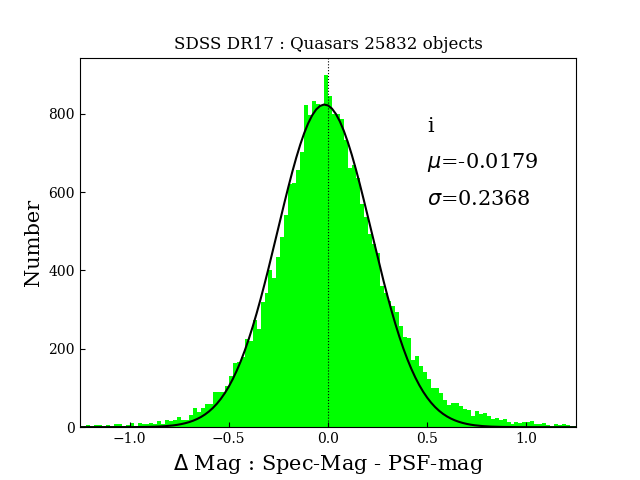
\includegraphics[angle=0,width=3.5cm]{figures/20220811_dmag_histogram_i_dr17quasars.png}
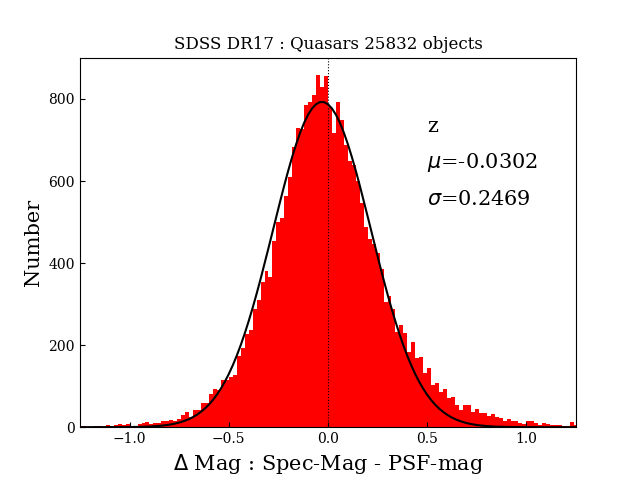
\includegraphics[angle=0,width=3.5cm]{figures/20220811_dmag_histogram_z_dr17quasars.png}
\caption{DR17 Quasar: Histogram of synthesized magnitude from spectra vs PSF magnitude.
u-band shows a large offset but it is due to spectral wavelength does not cover entire u-band region.}
\end{center}
\end{figure*}

\begin{figure*}%[ht]
\begin{center}
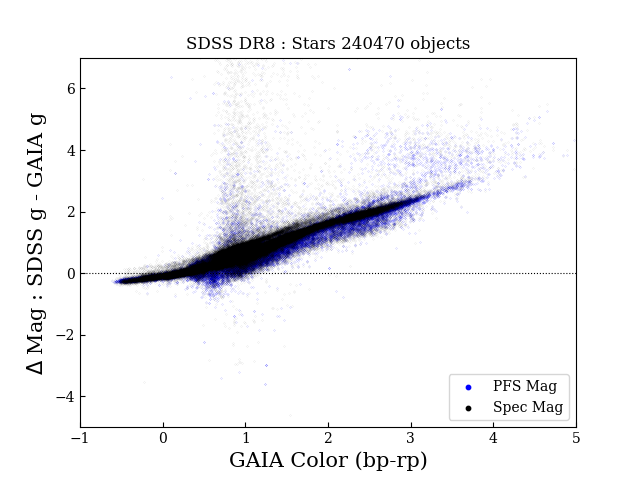
\includegraphics[angle=0,width=8.9cm]{figures/20220812_color_dmag_g_dr8star.png}
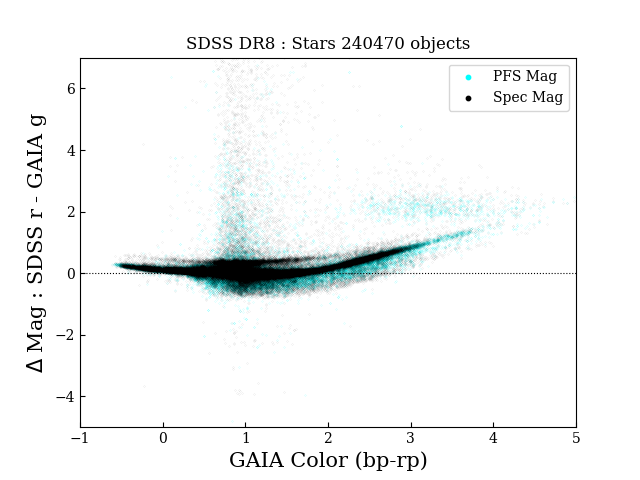
\includegraphics[angle=0,width=8.9cm]{figures/20220812_color_dmag_r_dr8star.png}
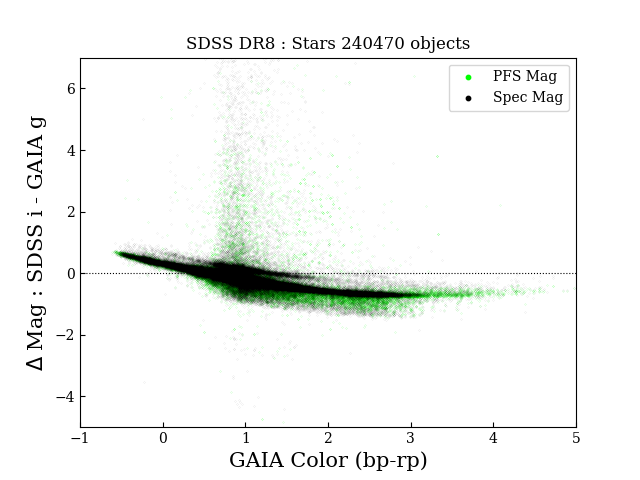
\includegraphics[angle=0,width=8.9cm]{figures/20220812_color_dmag_i_dr8star.png}
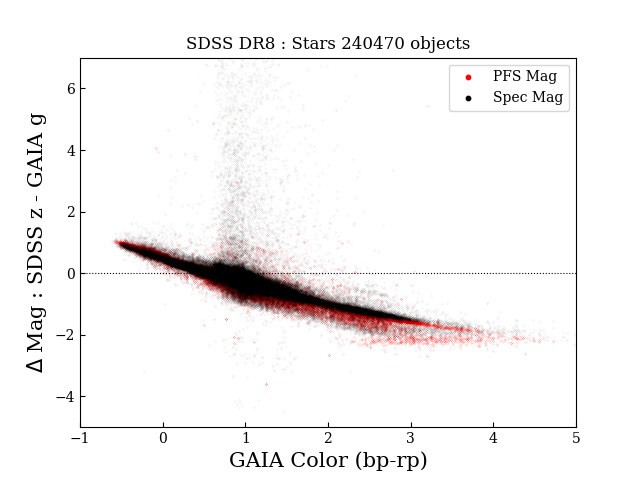
\includegraphics[angle=0,width=8.9cm]{figures/20220812_color_dmag_z_dr8star.png}
\caption{DR8 Star vs. GAIA g-mag: Color vs. $\Delta$M.  Testing GAIA mag color vs. SDSS mag - GAIA g-bmag.   GAIA g-mag is the whole filter system. SDSS-i band could be a good representative of GAIA-g.}
\end{center}
\end{figure*}

\begin{figure*}%[ht]
\begin{center}
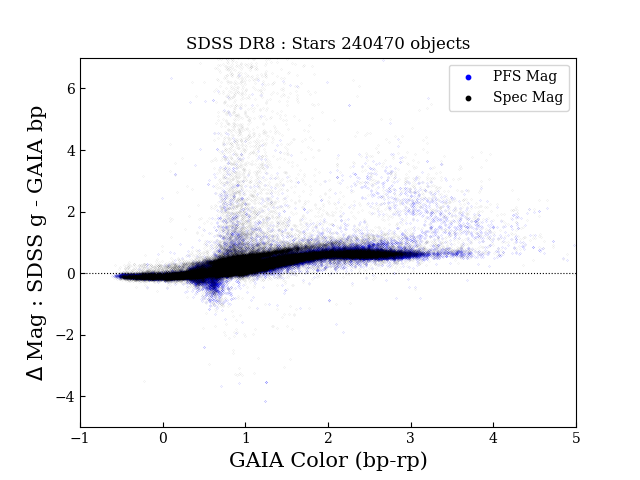
\includegraphics[angle=0,width=8.9cm]{figures/20220812_color_dmag_g_bp_dr8star.png}
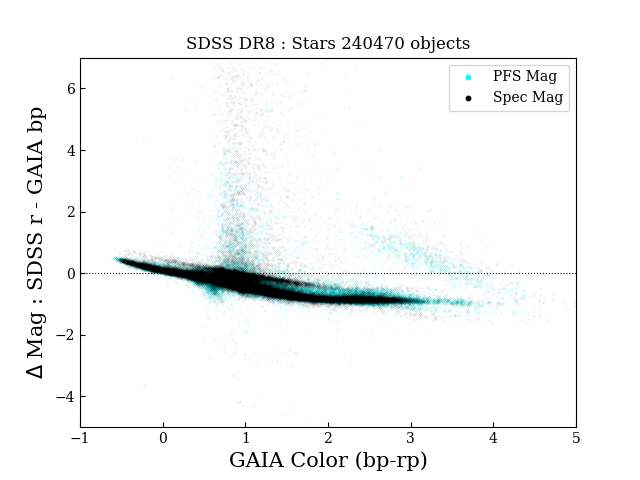
\includegraphics[angle=0,width=8.9cm]{figures/20220812_color_dmag_r_bp_dr8star.png}
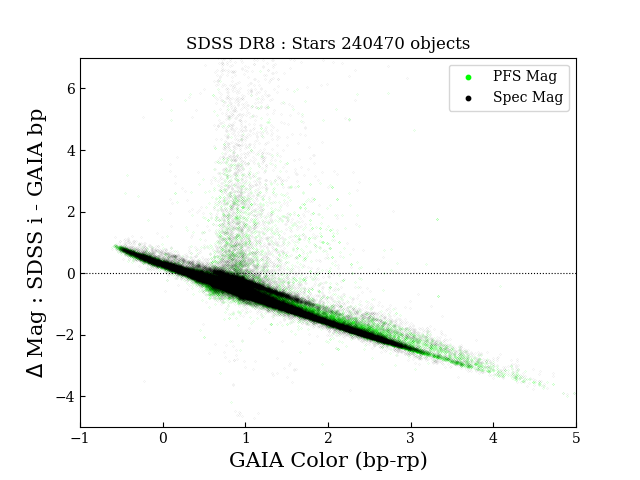
\includegraphics[angle=0,width=8.9cm]{figures/20220812_color_dmag_i_bp_dr8star.png}
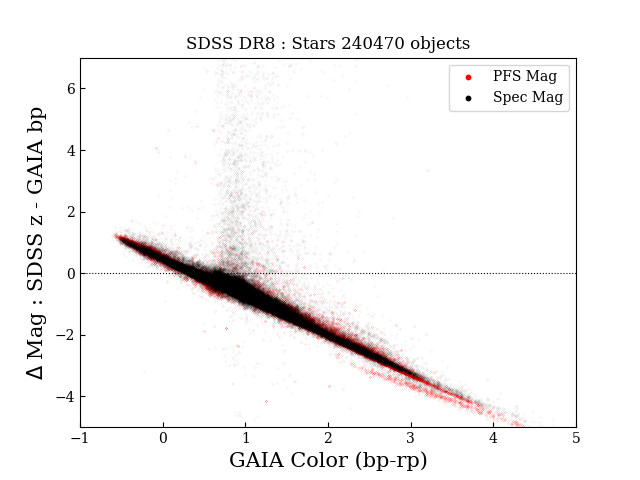
\includegraphics[angle=0,width=8.9cm]{figures/20220812_color_dmag_z_bp_dr8star.png}
\caption{DR8 Star vs. GAIA bp-mag : Color vs. $\Delta$M.  Note SDSS-g and SDSS-r are close to GAIA-bp}
\end{center}
\end{figure*}

\begin{figure*}%[ht]
\begin{center}
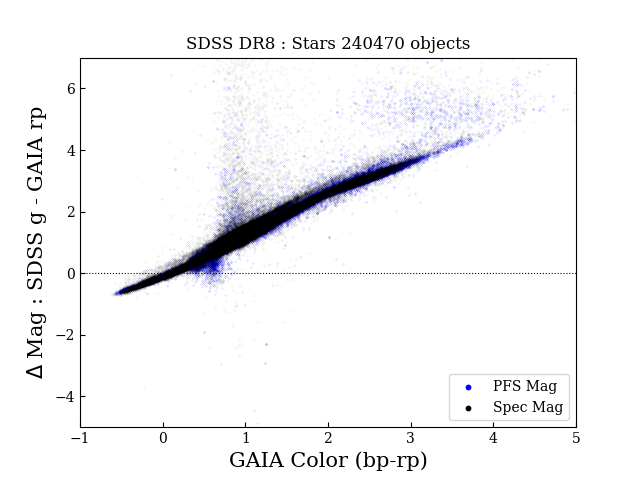
\includegraphics[angle=0,width=8.9cm]{figures/20220812_color_dmag_g_rp_dr8star.png}
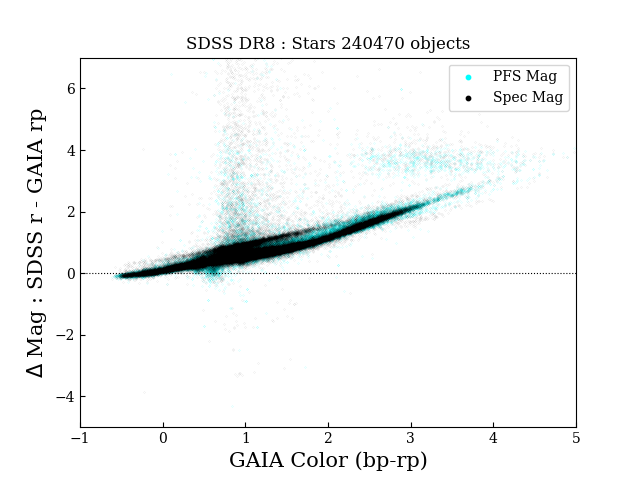
\includegraphics[angle=0,width=8.9cm]{figures/20220812_color_dmag_r_rp_dr8star.png}
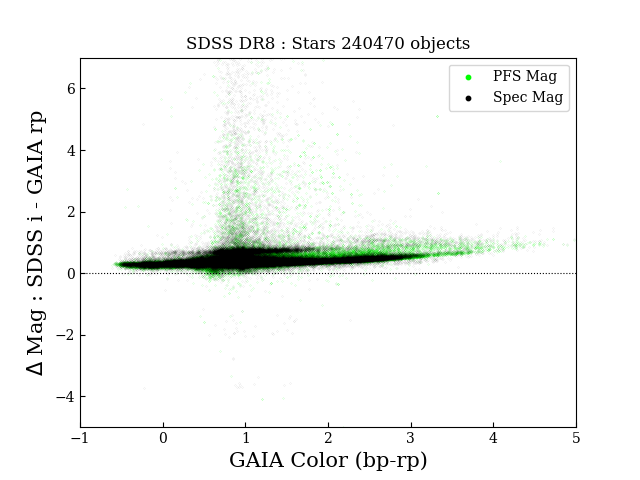
\includegraphics[angle=0,width=8.9cm]{figures/20220812_color_dmag_i_rp_dr8star.png}
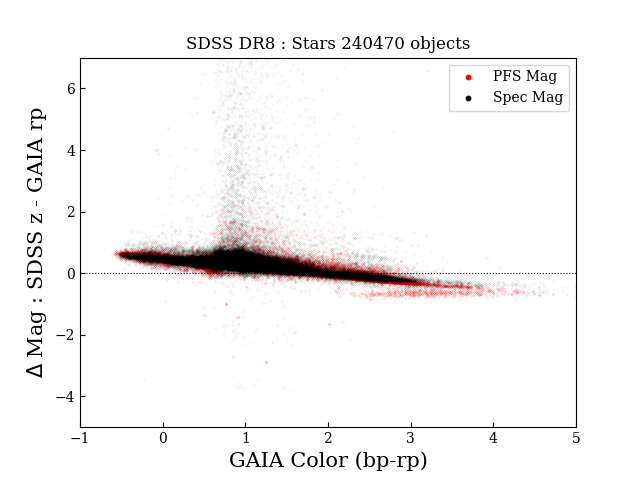
\includegraphics[angle=0,width=8.9cm]{figures/20220812_color_dmag_z_rp_dr8star.png}
\caption{DR8 Star vs. GAIA rp-mag : Color vs. $\Delta$M.  Note SDSS-i and SDSS-z are close to GAIA-rp as we expected.}
\end{center}
\end{figure*}

\begin{figure*}%[ht]
\begin{center}
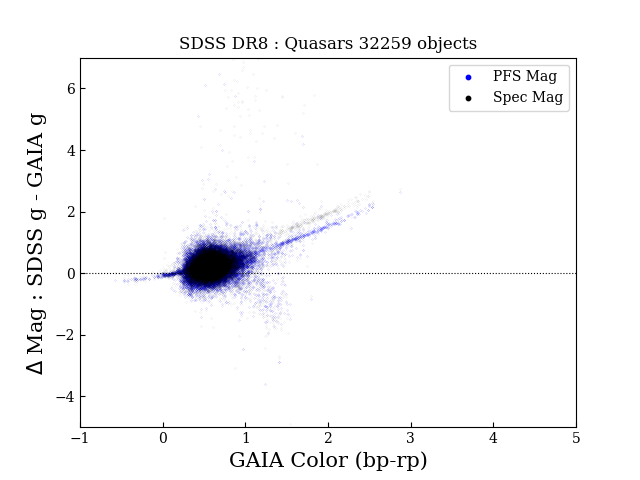
\includegraphics[angle=0,width=8.9cm]{figures/20220812_color_dmag_g_dr8quasar.png}
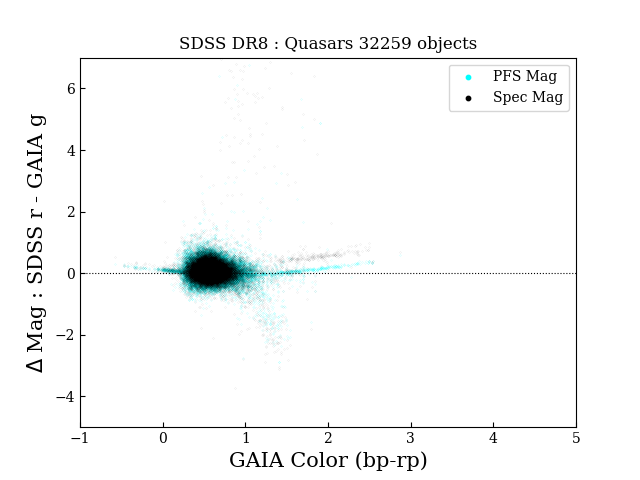
\includegraphics[angle=0,width=8.9cm]{figures/20220812_color_dmag_r_dr8quasar.png}
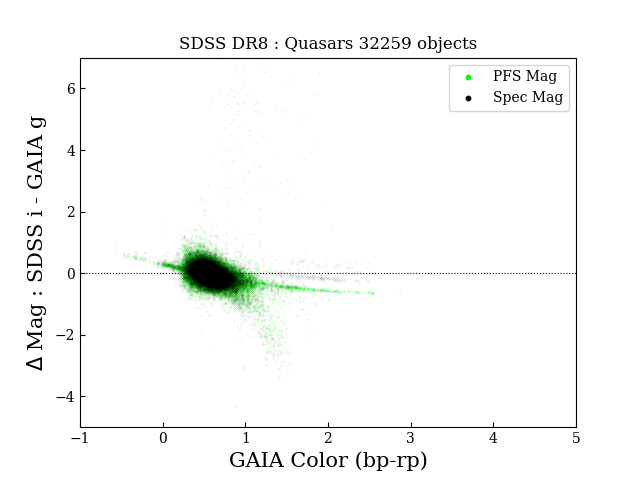
\includegraphics[angle=0,width=8.9cm]{figures/20220812_color_dmag_i_dr8quasar.png}
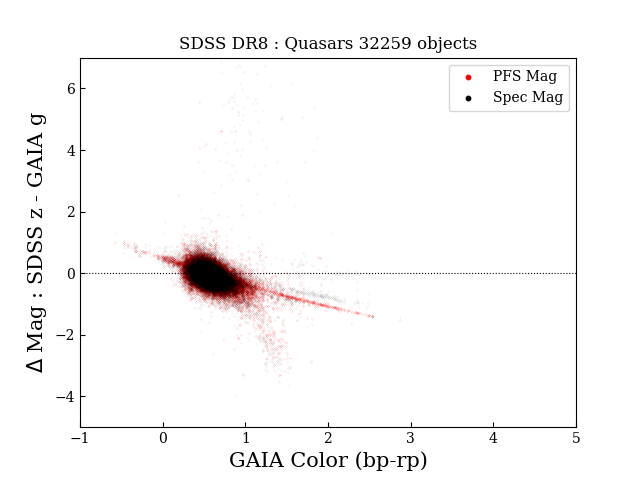
\includegraphics[angle=0,width=8.9cm]{figures/20220812_color_dmag_z_dr8quasar.png}
\caption{DR8 Quasar: Color vs. $\Delta$M.  The same plot but with Quasars.  The color range of quasars are limited.}
\end{center}
\end{figure*}

\begin{figure*}%[ht]
\begin{center}
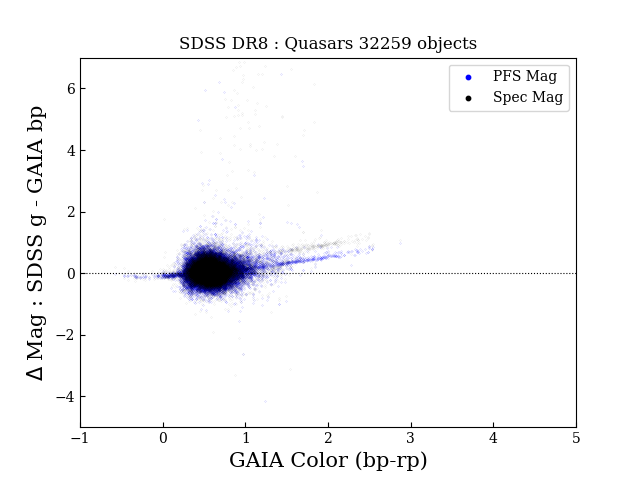
\includegraphics[angle=0,width=8.9cm]{figures/20220812_color_dmag_g_bp_dr8quasar.png}
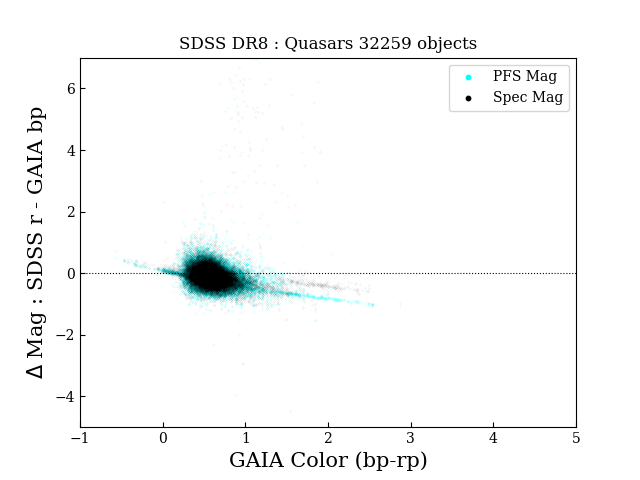
\includegraphics[angle=0,width=8.9cm]{figures/20220812_color_dmag_r_bp_dr8quasar.png}
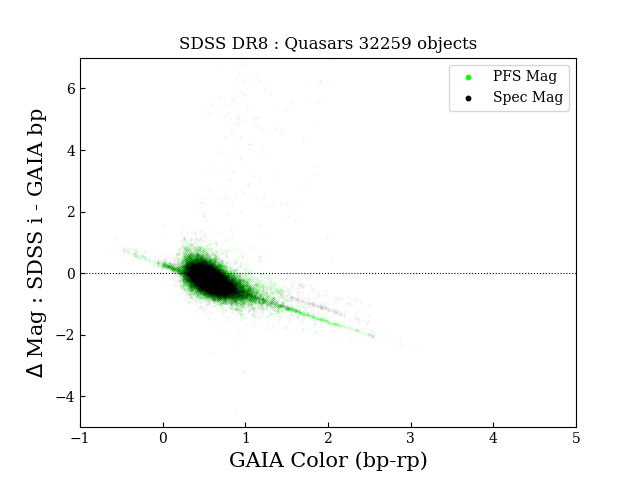
\includegraphics[angle=0,width=8.9cm]{figures/20220812_color_dmag_i_bp_dr8quasar.png}
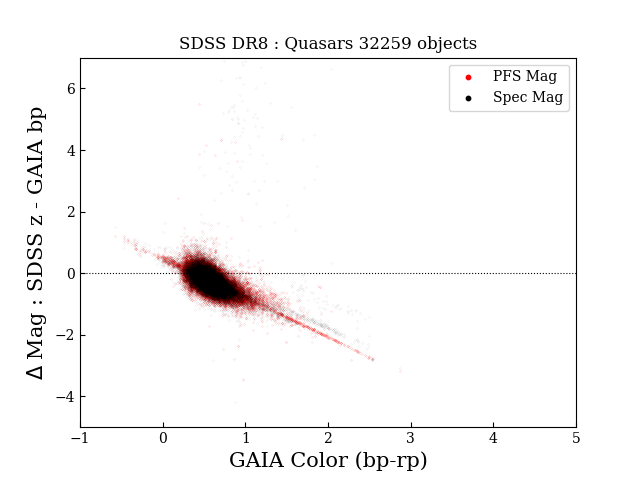
\includegraphics[angle=0,width=8.9cm]{figures/20220812_color_dmag_z_bp_dr8quasar.png}
\caption{DR8 Quasar vs. GAIA-bp mag: Color vs. $\Delta$M.  The same plot but with Quasars.  The color range of quasars are limited.}
\end{center}
\end{figure*}

\begin{figure*}%[ht]
\begin{center}
\includegraphics[angle=0,width=8.9cm]{figures/20220812_color_dmag_g_rp_dr8quasar.png}
\includegraphics[angle=0,width=8.9cm]{figures/20220812_color_dmag_r_rp_dr8quasar.png}
\includegraphics[angle=0,width=8.9cm]{figures/20220812_color_dmag_i_rp_dr8quasar.png}
\includegraphics[angle=0,width=8.9cm]{figures/20220812_color_dmag_z_rp_dr8quasar.png}
\caption{DR8 Quasar vs. GAIA-rp mag: Color vs. $\Delta$M.  The same plot but with Quasars.  The color range of quasars are limited.}
\end{center}
\end{figure*}

\begin{deluxetable*}{llllllllll}[ht]
%\rotate
\tablecaption{Host Galaxy Identification}
\tablehead{
\colhead{Survey}&
\colhead{z}&
\colhead{Filter}&
\colhead{Depth}&
\colhead{Radius(DLR)}&
\colhead{SNIa}&
\colhead{Hostless}&
\colhead{Fraction}&
\colhead{Reference}
}
\startdata
SDSS-II & 0.2$<$z$<$0.4 & r-band & 22.2 & 4R & 1236 & 198 & 16\% & \citet{sako18a} \\
PS-1    & 0.1$<$z$<$0.4 & i-band & 22.2 & 4R & &&& Scolnic \\
DES     & 0.1$<$z$<$0.7 & r-band & 25.8-26.3 & 7R & 206 & 4 & 1.9\% & \citet{smith20a} \\
DES     & 0.1$<$z$<$0.7 & r-band & 25.5-26.9 & 4R & 206 & 13 & 6.3\% & \citet{wiseman20a} \\
SNLS     & 0.3$<$z$<$0.7 & i-band & 24.0 & 4R & && 6.0\% & Sullivan\\
HSC     & 0.4$<$z$<$1.4 & r-band & 26.1(Wide), 27.7(UD) & TBD & &&& This work
\enddata
\end{deluxetable*}

%\begin{deluxetable}{lrrr}[ht]
%\rotate
\tablecaption{SDSS Hostless SN}
\tablehead{
\colhead{SN name}&
\colhead{RA}&
\colhead{DEC}&
\colhead{z}
}
\startdata
SN2005jn & 4.75348 & -0.28149 & 0.32045 \\
SN2007ml & 7.97272 & 0.13830 & 0.18563 \\
SN2006oi & 8.97105 & 0.25840 & 0.24857 \\
SN2007nd & 10.07840 & -1.03737 & 0.26856 \\
SN2007qp & 10.70177 & 0.37973 & 0.26357 \\
SN2005jc & 11.35171 & 1.07558 & 0.21163 \\
SN2007ix & 12.87867 & -0.94740 & 0.19867 \\
SN2007rq & 13.38379 & 0.90027 & 0.26559 \\
SN2006mn & 16.95163 & -0.10984 & 0.29761 \\
SN2005go & 17.70495 & 1.00794 & 0.26405 \\
SN2006nj & 21.11762 & 0.07439 & 0.38857 \\
SN2007jj & 26.36137 & -0.01942 & 0.23381 \\
SN2007qy & 28.81367 & 0.64310 & 0.22786 \\
SN2006nw & 30.73313 & -0.53387 & 0.15596 \\
SN2007je & 32.94712 & -0.91243 & 0.15999 \\
SN2005ey & 34.27287 & 0.28030 & 0.14702 \\
SN2005jd & 34.27586 & 0.53483 & 0.31288 \\
SN2007rl & 35.38779 & -0.37493 & 0.32290 \\
SN2007rm & 35.43787 & 0.86446 & 0.30092 \\
SN2006fk & 330.25553 & 0.71624 & 0.17063 \\
SN2006pi & 330.81918 & -0.60684 & 0.36640 \\
SN2007se & 333.15459 & 0.79672 & 0.17360 \\
SN2005gs & 333.29273 & 1.05054 & 0.24961 \\
SN2006nu & 340.82916 & 0.26291 & 0.19654 \\
SN2006hf & 345.21873 & -0.98114 & 0.20852 \\
SN2007jo & 347.55242 & -0.93141 & 0.18854 \\
SN2006gn & 347.82678 & 0.50461 & 0.10264 \\
SN2006hk & 350.12309 & -1.15785 & 0.28742 \\
SN2007lw & 354.20377 & -0.78223 & 0.28543 \\
SN2007pj & 357.29456 & 0.79788 & 0.35236 \\
SN2005ja & 358.96933 & 0.87697 & 0.32640 \\
SN2007mk & 359.07222 & -0.50587 & 0.17558 
\enddata
\end{deluxetable*}


%\begin{deluxetable}{lrrr}[ht]
%\rotate
\tablecaption{SDSS Hostless SN}
\tablehead{
\colhead{SN name}&
\colhead{RA}&
\colhead{DEC}&
\colhead{z}
}
\startdata
SN2005jn&00:21:34.592&-00:00:15.22&0.32045\\
SN2007ml&00:34:27.269&+00:24:49.47&0.18563\\
SN2006oi&00:38:26.896&+00:31:59.16&0.24857\\
SN2007nd&00:42:52.395&-00:45:48.91&0.26856\\
SN2007qp&00:45:22.309&+00:39:10.61&0.26357\\
SN2005jc&00:47:58.465&+01:20:53.43&0.21163\\
SN2007ix&00:54:04.432&-00:40:35.03&0.19867\\
SN2007rq&00:56:06.163&+01:10:14.51&0.26559\\
SN2006mn&01:10:22.165&+00:09:21.46&0.29761\\
SN2005go&01:13:23.365&+01:16:21.47&0.26405\\
SN2006nj&01:27:02.080&+00:20:00.55&0.38857\\
SN2007jj&01:48:00.546&+00:13:45.46&0.23381\\
SN2007qy&01:57:49.477&+00:53:10.45&0.22786\\
SN2006nw&02:05:29.463&-00:17:43.46&0.15596\\
SN2007je&02:14:20.560&-00:40:46.87&0.15999\\
SN2005ey&02:19:39.510&+00:30:33.99&0.14702\\
SN2005jd&02:19:40.396&+00:45:50.26&0.31288\\
SN2007rl&02:24:06.651&-00:08:56.05&0.32290\\
SN2007rm&02:24:19.514&+01:05:25.22&0.30092\\
SN2006fk&22:03:34.631&+00:57:31.27&0.17063\\
SN2006pi&22:05:50.659&-00:21:47.00&0.36640\\
SN2007se&22:15:10.404&+01:02:44.78&0.17360\\
SN2005gs&22:15:43.429&+01:17:59.60&0.24961\\
SN2006nu&22:45:52.630&+00:31:34.80&0.19654\\
SN2006hf&23:03:26.520&-00:42:41.77&0.20852\\
SN2007jo&23:12:46.553&-00:39:33.36&0.18854\\
SN2006gn&23:13:52.051&+00:46:37.30&0.10264\\
SN2006hk&23:23:03.516&-00:53:00.09&0.28742\\
SN2007lw&23:39:22.752&-00:30:18.52&0.28543\\
SN2007pj&23:51:44.423&+01:04:33.57&0.35236\\
SN2005ja&23:58:26.398&+01:09:19.08&0.32640\\
SN2007mk&23:58:51.111&-00:13:39.11&0.17558
\enddata
\end{deluxetable}


\section{Data}


\subsection{SDSS-II Supernova Survey}

\subsection{Subaru HSC SSP Data}


%\begin{figure*}%[ht]
\begin{center}
\includegraphics[angle=0,width=4.0cm]{figures/thumbnails/SN2005ey.png}
\includegraphics[angle=0,width=4.0cm]{figures/thumbnails/SN2005go.png}
\includegraphics[angle=0,width=4.0cm]{figures/thumbnails/SN2005gs.png}
\includegraphics[angle=0,width=4.0cm]{figures/thumbnails/SN2005ja.png}
\includegraphics[angle=0,width=4.0cm]{figures/thumbnails/SN2005jc.png}
\includegraphics[angle=0,width=4.0cm]{figures/thumbnails/SN2005jd.png}
\includegraphics[angle=0,width=4.0cm]{figures/thumbnails/SN2005jn.png}
\includegraphics[angle=0,width=4.0cm]{figures/thumbnails/SN2006fk.png}
\includegraphics[angle=0,width=4.0cm]{figures/thumbnails/SN2006gn.png}
\includegraphics[angle=0,width=4.0cm]{figures/thumbnails/SN2006hf.png}
\includegraphics[angle=0,width=4.0cm]{figures/thumbnails/SN2006hk.png}
\includegraphics[angle=0,width=4.0cm]{figures/thumbnails/SN2006mn.png}
\includegraphics[angle=0,width=4.0cm]{figures/thumbnails/SN2006nj.png}
\includegraphics[angle=0,width=4.0cm]{figures/thumbnails/SN2006nu.png}
\includegraphics[angle=0,width=4.0cm]{figures/thumbnails/SN2006nw.png}
\includegraphics[angle=0,width=4.0cm]{figures/thumbnails/SN2006oi.png}
\includegraphics[angle=0,width=4.0cm]{figures/thumbnails/SN2006pi.png}
\includegraphics[angle=0,width=4.0cm]{figures/thumbnails/SN2007ix.png}
\includegraphics[angle=0,width=4.0cm]{figures/thumbnails/SN2007je.png}
\includegraphics[angle=0,width=4.0cm]{figures/thumbnails/SN2007jj.png}
\includegraphics[angle=0,width=4.0cm]{figures/thumbnails/SN2007jo.png}
\includegraphics[angle=0,width=4.0cm]{figures/thumbnails/SN2007lw.png}
\includegraphics[angle=0,width=4.0cm]{figures/thumbnails/SN2007mk.png}
\includegraphics[angle=0,width=4.0cm]{figures/thumbnails/SN2007ml.png}
\includegraphics[angle=0,width=4.0cm]{figures/thumbnails/SN2007nd.png}
\includegraphics[angle=0,width=4.0cm]{figures/thumbnails/SN2007pj.png}
\includegraphics[angle=0,width=4.0cm]{figures/thumbnails/SN2007qp.png}
\includegraphics[angle=0,width=4.0cm]{figures/thumbnails/SN2007qy.png}
\includegraphics[angle=0,width=4.0cm]{figures/thumbnails/SN2007rl.png}
\includegraphics[angle=0,width=4.0cm]{figures/thumbnails/SN2007rm.png}
\includegraphics[angle=0,width=4.0cm]{figures/thumbnails/SN2007rq.png}
\includegraphics[angle=0,width=4.0cm]{figures/thumbnails/SN2007se.png}
\end{center}
\end{figure*}



\section{Host Galaxy Identification}
We use 

%HSC Transient survey is being conducted in deep and ultra-deep region, but for this study, we use the HSC SSP Wide field data.

\section{Table}

%There is a theory which states that if ever anyone discovers exactly what the Universe is for and why it is here, it will instantly disappear and be replaced by something even more bizarre and inexplicable.
%There is another theory which states that this has already happened.

%\begin{figure}[h!]
%\centering
%\includegraphics[scale=1.7]{universe}
%\caption{The Universe}
%\label{fig:universe}
%\end{figure}

\section{Conclusion}
``I always thought something was fundamentally wrong with the universe''
%``I always thought something was fundamentally wrong with the universe'' \citep{adams1995hitchhiker}

%\bibliographystyle{plain}
%\bibliography{archive,references}
\clearpage
\bibliography{archive}
\end{document}

